%\documentclass[letter,11pt]{article} % Tamaño de página y letra, tipo de documento
%\usepackage[top = 2.0cm, bottom = 2.0cm, left = 2.0cm, right = 2.0cm]{geometry}

\documentclass[letter,11pt]{article}
\usepackage[top=2.0cm, bottom=2.0cm, left=2.0cm, right=2.0cm]{geometry}

% Configuración de Fira Sans para TODO el documento
\usepackage[sfdefault]{FiraSans} % Fuente principal
\usepackage{FiraMono}

%% Comandos para codificación de archivo
%\usepackage[T1]{fontenc}
\usepackage[utf8]{inputenc}
% Se configura diccionario en español y en entorno de tablas aparecerá el nombre Tabla x
\usepackage[spanish,es-tabla]{babel}
% Se utilizará el punto decimal en lugar de coma para definir números con decimales
\spanishdecimal{.}
%%%%%%%%%%%%%%%%%%%%%%%%%%%%%%%%%%%%%%%%%%%%%%%%
%% Bibliotecas útiles %%
\usepackage{multirow} % Múltiples renglones
\usepackage{multicol} % Múltiples columnas
\usepackage{booktabs} % For even nicer tables.
\usepackage{graphicx} % Necesario para agregar figuras
\usepackage{setspace}  % Quita sangría de inicio de párrafos
\setlength{\parindent}{0in}
\usepackage{float} % Colocar figuras donde se indique
\usepackage{fancyhdr} % Da formato a encabezados
\usepackage{amsmath,mathtools,amsfonts,amssymb} % Para agregar símbolos matemáticos
\usepackage{epstopdf} % Para agregar figuras en formato eps
\usepackage{xcolor} % Para agregar color a texto y ecuaciones
\usepackage{fancyvrb}  % Necesario para incluir código de Matlab
\usepackage{amsmath}
\usepackage{pdfpages}
\usepackage{graphicx}
\usepackage{enumitem}
\usepackage{tocloft}
\usepackage{booktabs}
\usepackage{hyperref}
\usepackage{array}
\usepackage{tcolorbox}
\usepackage{lmodern}
\usepackage{tikz}
\usepackage{geometry}
\usepackage{setspace}
\usepackage{anyfontsize}
\usepackage{makecell}
\usepackage[normalem]{ulem}
\hypersetup{
	colorlinks=false,
	pdfborder={0 0 0}
}
\usepackage{listings}
\definecolor{backcolour}{rgb}{0.95,0.95,0.92}

\lstdefinestyle{bashstyle}{
	backgroundcolor=\color{backcolour},
	basicstyle=\ttfamily\small,
	numbers=left,
	numberstyle=\tiny\color{gray},
	frame=single,
	tabsize=4,
	breaklines=true,
	captionpos=b,
	keywordstyle=\color{blue},
	commentstyle=\color{green!50!black},
	stringstyle=\color{red},
	morekeywords={sudo, apt, git, echo, if, then, else, fi, for, do, done, while, until, case, esac, function, cd, ls, mkdir, rm, cp, mv, chmod, grep, find, awk, sed},
	literate=*
	{_} {\textunderscore}{1}  % ← Esto arregla el guión bajo
	{\$} {\textdollar}{1}
	{\#} {\#}{1}
	{\{} {\{}{1}
	{\}} {\}}{1}
	{>} {\textgreater}{1}
	{<} {\textless}{1}
	{|} {\textbar}{1}
	{~} {\textasciitilde}{1}
	{\`} {\`}{1}
	{\^} {\^{}}{1}
	{*} {\ast}{1}
}

% Definir estilo sutil con bordes redondeados
\newtcbox{\highlight}[1][]{%
	nobeforeafter,
	tcbox raise base,
	arc=3pt,
	boxrule=0pt,
	left=2pt,
	right=2pt,
	top=1pt,
	bottom=1pt,
	colback=yellow!20!white,
	colframe=white,
	#1
}

% Colores institucionales UNAM
\definecolor{unamblue}{RGB}{0,51,102}
\definecolor{unamgold}{RGB}{153,126,48}
\definecolor{myred}{HTML}{911010}
\definecolor{myblue}{HTML}{142966}
\definecolor{myaqua}{HTML}{1EA69A}



%% Encabezado y pie de página %%
\pagestyle{fancy}  
\fancyhf{} 
\renewcommand{\headrule}{\hbox to\headwidth{\color{black}\leaders\hrule height \headrulewidth\hfill}}
\renewcommand{\headrulewidth}{0.4pt} % Línea del encabezado
\fancyhead[L]{\color{black}\small{Computación Gráfica e Interacción Humano-Computadora}}
\fancyhead[R]{\color{black}\small{Prototipo}}
\fancyfoot[R]{\small\thepage}

%%%%%%%%%%%%%%%%%%%%%%%%%%%%%%%%%%%%%%%%%%%%%%%%
%% Aquí comienza la edición del documento

\begin{document}
\thispagestyle{empty} % Sin encabezado la primera página
%% Datos para la primera página
\begin{center}
	\vspace{0.8cm}
	\begin{minipage}{0.125\textwidth}
		\centering
		
\includegraphics[width=\textwidth]{UNAM}
	\end{minipage}
	\hfill
	\begin{minipage}{0.7\textwidth}
		\centering
		{\color{black}\fontsize{16}{18}\selectfont
			\textbf{UNIVERSIDAD NACIONAL AUTÓNOMA DE MÉXICO} \\
			\vspace{0.3cm}
			\textbf{FACULTAD DE INGENIERÍA} \\
			\vspace{0.3cm}
			\textbf{COMPUTACIÓN GRÁFICA E INTERACCIÓN HUMANO-COMPUTADORA} \\
			\vspace{0.3cm}
			\textbf{SEMESTRE 2027 - 1}
		}
	\end{minipage}
	\hfill
	\begin{minipage}{0.125\textwidth}
		\centering
		
\includegraphics[width=\textwidth]{UNAM_INGENIERIA}
	\end{minipage}
	
	\vspace{2cm}
	
	\begin{tikzpicture}
		%\draw[unamgold, line width=1pt] (0,0) -- (0.2\textwidth,0);
		%\draw[unamblue, line width=1pt] (0.2\textwidth,0) -- (0.8\textwidth,0);
		\draw[black, line width=1.5pt] (2\textwidth,0) -- (\textwidth,0);
	\end{tikzpicture}
	
	\vspace{2cm}
	
	{\color{black}\fontsize{18}{20}\selectfont
		\textbf{PROTOTIPO DE PROYECTO FINAL} \\
		\vspace{0.5cm}
	}
	
	\vspace{1.5cm}
	
	{\color{black}\fontsize{14}{16}\selectfont
		\begin{tabular}{l r l}
			\textbf{ALUMNOS} & \textit{Basilio Illescas Andrés} & \textit{Project Owner} \\[0.3cm]
			 & \textit{Trejo Olvera Emmanuel} & \textit{Scrum Master} \\[0.3cm]
			 & \textit{Pérez Olvera Alexis Abraham} & \textit{Developer} \\[0.3cm]
			 & \textit{Cruz Macedo Samuel Santiago} & \textit{Developer} \\[0.3cm]
			\textbf{PROFESOR} & \textit{Ing. José Ramón Pérez Athié} & \\[0.3cm]
			\textbf{GRUPO} & \textit{04} & \\[0.3cm]
		\end{tabular}
	}
	
	\vfill
	
	{\color{black}\fontsize{12}{14}\selectfont
		Ciudad Universitaria, CDMX \hfill \today
	}
\end{center}
\newpage

%\begin{tabular} {p{9cm} p{8cm}}
%	\multirow{-2}{*}{
\includegraphics[scale=0.11]{UNAM_INGENIERIA}} &
%	\hfill \textit{Universidad Nacional Autónoma de México} \\
% & \hfill \textit{Facultad de Ingeniería} \\
% & \hfill {\large \bf LAB. BASES DE DATOS} \\
% & \hfill {\large \bf PRÁCTICA 01 - REPORTE} \\
% & \\
%\hline % \hline produce una línea horizontal
%\end{tabular} 

\newpage

\begin{center}
	{\LARGE\bfseries Prototipo de altar de Día de Muertos}\par
	\vspace{0.2cm}
\end{center}

\section*{Descripción del prototipo}
El proyecto consiste en una escena tridimensional de un altar de Día de
Muertos elaborada en Blender. Este primer prototipo permite definir la
distribución de los elementos, sus proporciones y el encuadre antes de
realizar el modelado detallado. La estructura se compone de tres niveles
rectangulares, cada uno más pequeño que el anterior.

% Se incluye el render cuando el compilador tiene acceso a los archivos locales.
% El recuadro permite previsualizar el texto en editores sin soporte de adjuntos.
\begin{figure}[ht]
	\centering
	\IfFileExists{altar_prototipo.png}{%
		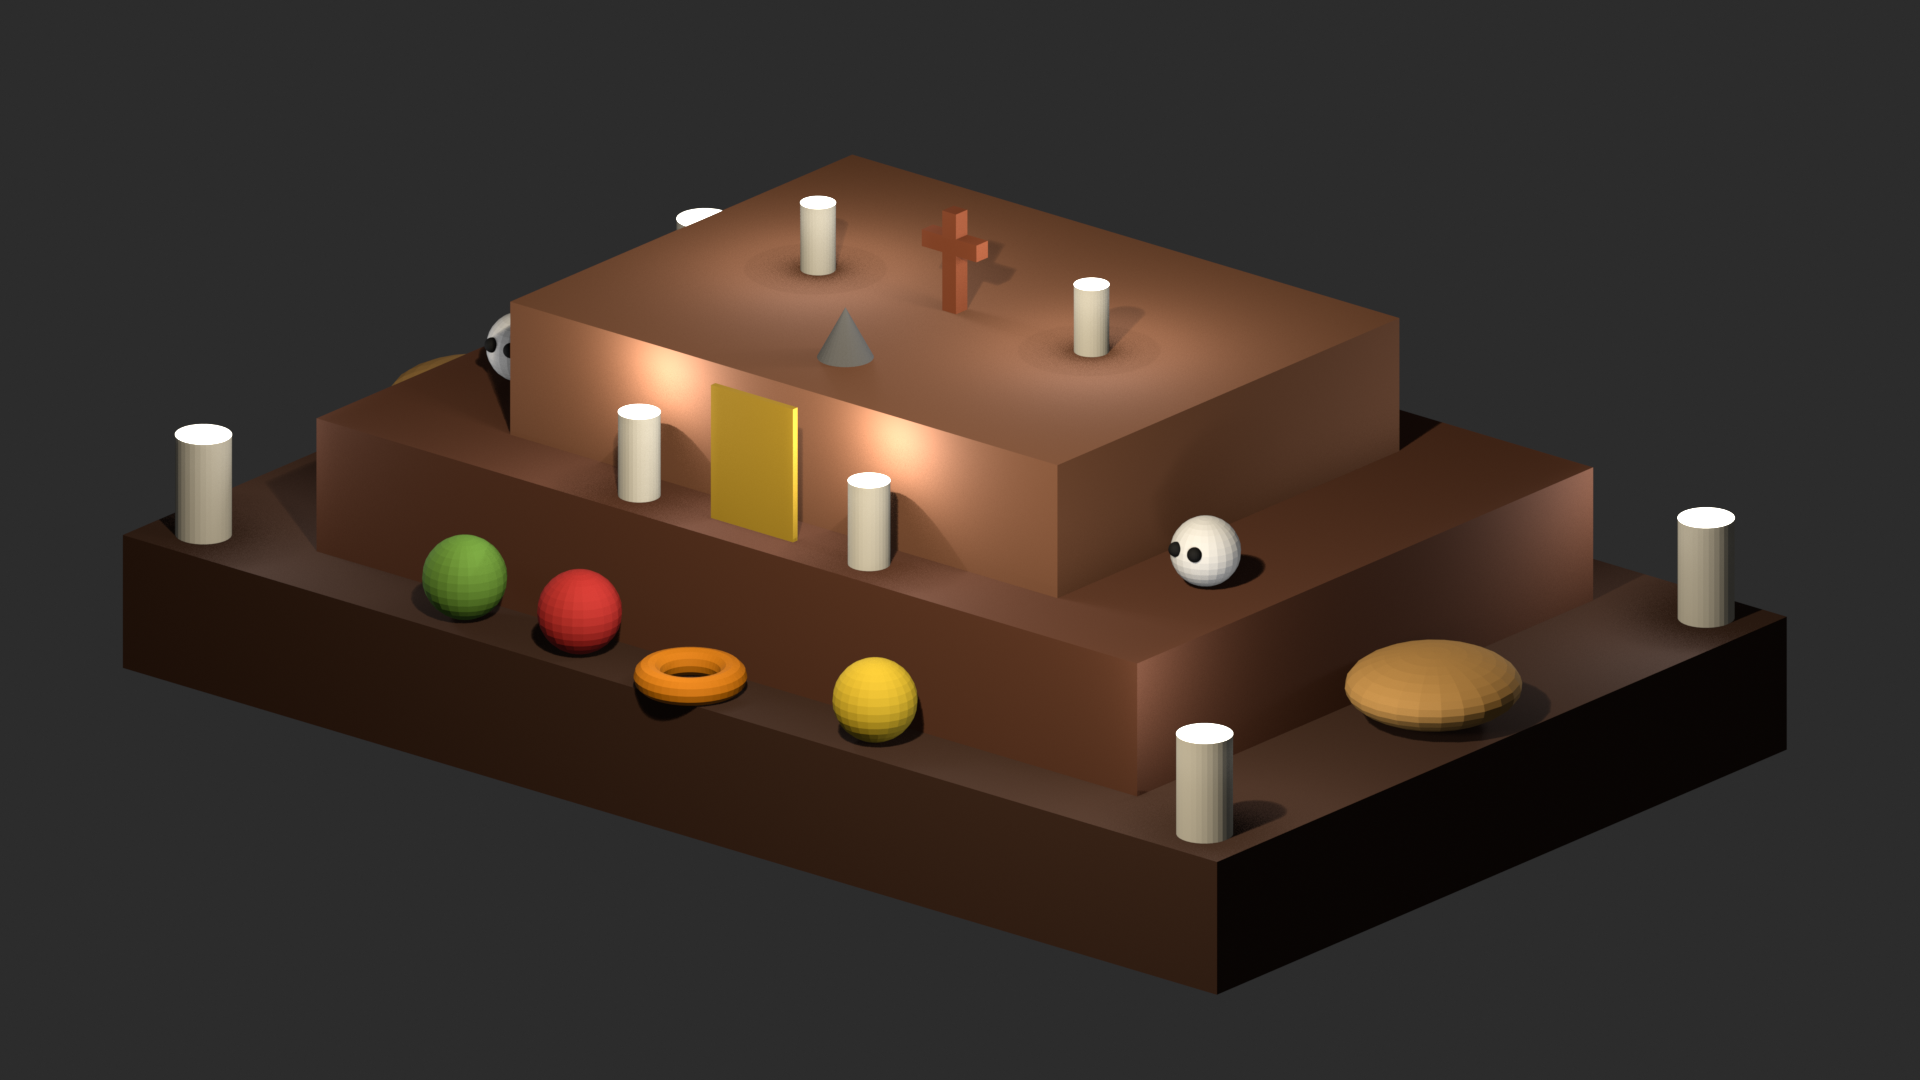
\includegraphics[width=0.94\textwidth]{altar_prototipo.png}%
	}{%
		\IfFileExists{final-project-cgih-c/Prototipo/altar_prototipo.png}{%
			\includegraphics[width=0.94\textwidth]{final-project-cgih-c/Prototipo/altar_prototipo.png}%
		}{%
			\fbox{\parbox[c][6.8cm][c]{0.90\textwidth}{\centering
					Espacio para el render del prototipo.\\[0.3cm]
					Archivo: \texttt{altar\_prototipo.png}}}%
		}%
	}
	\caption{Vista general del prototipo del altar, construido con primitivas y colores planos.}
\end{figure}

\section*{Elementos representados}
La base contiene velas, panes de muerto, frutas y una representación
simplificada de una flor de cempasúchil. En el nivel intermedio se ubican
calaveritas de azúcar, dos velas y una placa dorada que indica la posición
del futuro marco con retrato. El nivel superior contiene una cruz, dos
velas y un incensario.

Por ahora se utilizan cubos, cilindros, esferas, un toro y un cono con
materiales de colores planos. La iluminación cálida y el fondo gris oscuro
ayudan a distinguir los volúmenes y a visualizar la composición general.

\section*{Propuesta para la versión final}
Se propone conservar la estructura de tres niveles y sustituir las formas
más simples por modelos reconocibles: panes con sus adornos característicos,
calaveritas con mandíbula y detalles decorativos, flores con pétalos, frutas
con tallos, papel picado y un incensario con una animación de humo. Las velas incorporarían mechas y
llamas, y la placa dorada representaria marcos con retrato.

El resultado esperado es un altar más detallado y expresivo, manteniendo
una estética estilizada y la paleta cálida del prototipo. También se
ajustarían la separación entre las ofrendas, el encuadre y la iluminación
para que los elementos principales sean visibles y las velas contribuyan
a la ambientación de la escena.
			
\end{document}